\documentclass[12pt,a4paper]{book}

\setcounter{tocdepth}{3}

\usepackage[utf8]{inputenc}
\usepackage[french]{babel}
\usepackage[T1]{fontenc}
\usepackage{graphicx}
\usepackage{fullpage}
\usepackage{url}
\usepackage{caption}
\usepackage{subcaption}

\usepackage{amsmath}
\usepackage{amsfonts}
\usepackage{dsfont}
\usepackage{amssymb}

\usepackage{comment}

\usepackage{amsthm}
\newtheorem{env_definition}{Définition}
\newtheorem{formule}{Formule}
\newtheorem{annexe}{Annexe}

\usepackage[colored]{shadethm}
\definecolor{shadethmcolor}{rgb}{1,0.871,0.890}% couleur du fond
\definecolor{shaderulecolor}{rgb}{0.651,0.074,0.090}% couleur de l'encadré
\newshadetheorem{env_proposition}{Proposition}
\newshadetheorem{env_lemme}{Lemme}
\newshadetheorem{theorem}{Théorème}

\newcommand{\R}{\mathbb{R}}

\renewcommand\thesection{\Roman{section}}

\newcommand{\E}{\mathbb{E}}
\newcommand{\p}{\mathbb{P}}
\newcommand{\1}{\mathds{1}}

\DeclareMathOperator*{\argmin}{arg\!\min}


\usepackage{pythonhighlight}
%\usepackage[margin=0.5in]{geometry}
\usepackage{color, colortbl}
\usepackage{xcolor}
\usepackage{graphicx}
\usepackage{caption}


\definecolor{Gray}{gray}{0.9}
\definecolor{DarkGray}{gray}{0.5}
\definecolor{LightCyan}{rgb}{0.88,1,1}
\definecolor{yellow}{rgb}{1,1,0}

\begin{document}



% Page de garde
	
\begin{titlepage}
	\thispagestyle{empty}
	\begin{center}
	
    
\includegraphics[scale=1.]{Logo}  
	\vspace{1 cm}

	
	\vspace{0.7 cm}
	\textbf{{\fontsize{26}{34} \selectfont Prédiction de la Production de Bière en Australie }}\\
	\vspace{1 cm}
	 
	
	\vspace{1.5 cm}
	{\fontsize{15}{25} \selectfont Par : \\
		\item Philippine RENAUDIN
		\item Elvina EURY
	}\\
	\vspace{0.5 cm}
	{\fontsize{15}{25} \selectfont Master 2 Mathématiques et Applications}\\
	{\fontsize{15}{25} \selectfont Parcours Data Science}\\
	\vspace{1 cm}
	{\fontsize{10}{25} \selectfont Sous la direction de M. Frédéric Proia}
	\vspace{1.5 cm}

	{\fontsize{20}{30} \selectfont 2020-2021}\\
	
	\end{center}
\end{titlepage}

\thispagestyle{empty}
\newpage


% Table des matières


% Description du sujet

\newpage
\setcounter{page}{1}

\noindent
{\LARGE \textbf{Introduction}}
\vspace{5 mm}

%===============================================================================

L'objectif de cet étude est de prédire la production de bière en Australie pour les trois prochaines années à partir de séries chronologiques. La production de bière est une variable endogène car elle est dépendante de d'autres facteurs comme le climat. Nous nous basons sur des données mensuelles, de janvier 1956 à août 1995. Comme il est difficile de visuellement discerner le modèle multiplicatif de l'additif nous analysons à la fois le modèle initial et le modèle transformée. Notre approche de vise en premier lieu à transformer les données, à éliminer la périodicité et la tendance avant de rendre le processus stationnaire. Puis des tests statistiques sont effectués sur les résidus afin de cibler les modèles les plus robustes. Finalement, nous utilisons les modèles choisis afin de prédire la production de bière sur les trois prochaines années. 
A COMPLETER/ MODIFIER...


\vspace{15 mm}

%===============================================================================

\noindent
{\LARGE \textbf{Méthologie}}
\vspace{5 mm}


\subsection{Analyse initiale}

Les séries chronologiques ont 3 composantes principales: La tendance (T), qui décrit les mouvement à long terme, la périodicité (S), qui est cyclique, et les fluctuations ($\epsilon$).
\vspace{5 mm}
Nous débutons notre approche en faisant une analyse visuelle des séries chronologiques. 

À première vue nous voyons que nos séries sont non-stationnaire avec une tendance et une périodicité annuelle. Cette dernière est d'ailleurs confirmé sur les sorties ACF et PACF des séries initiales. Il est dur à dire si la tendance est quadratique ou linéaire. Nous nous baserons sur des tests supplémentaires pour être sûr.  De plus, nous remarquons un accroissement subtile de la saisonnalité, nous laissant un doute quant à la nature multiplicative ou additive du modèle. Nous avons ainsi décidé de comparer les résultats obtenus des séries initiales, avec les résultats du logarithme des séries. 

\begin{figure}[h]
	\begin{subfigure}{.5\textwidth}
  		\centering
    	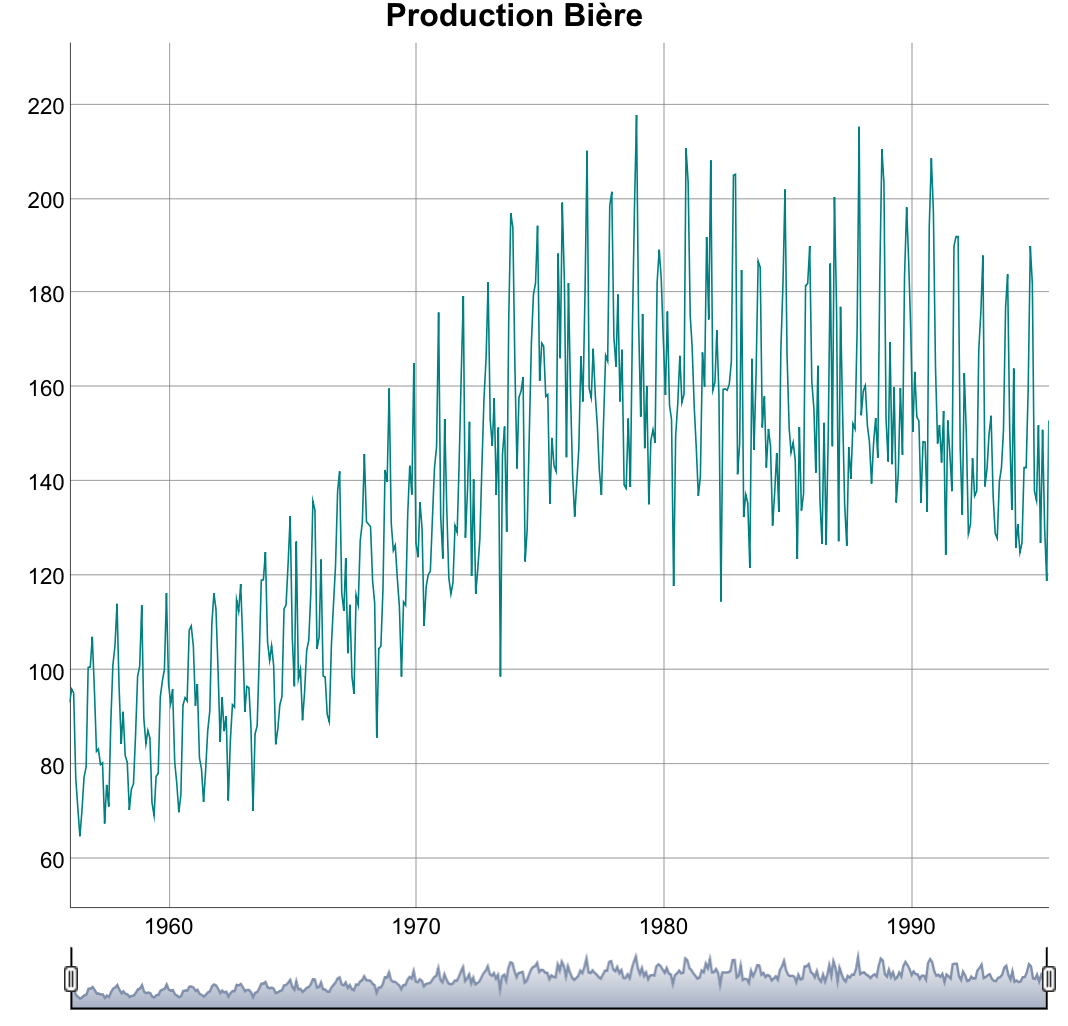
\includegraphics[scale=0.2]{plot_beer}  
    	\caption{Série Initiale}
    	\label{fig:sub1}
    \end{subfigure}
    \begin{subfigure}{.5\textwidth}
    	\centering
    	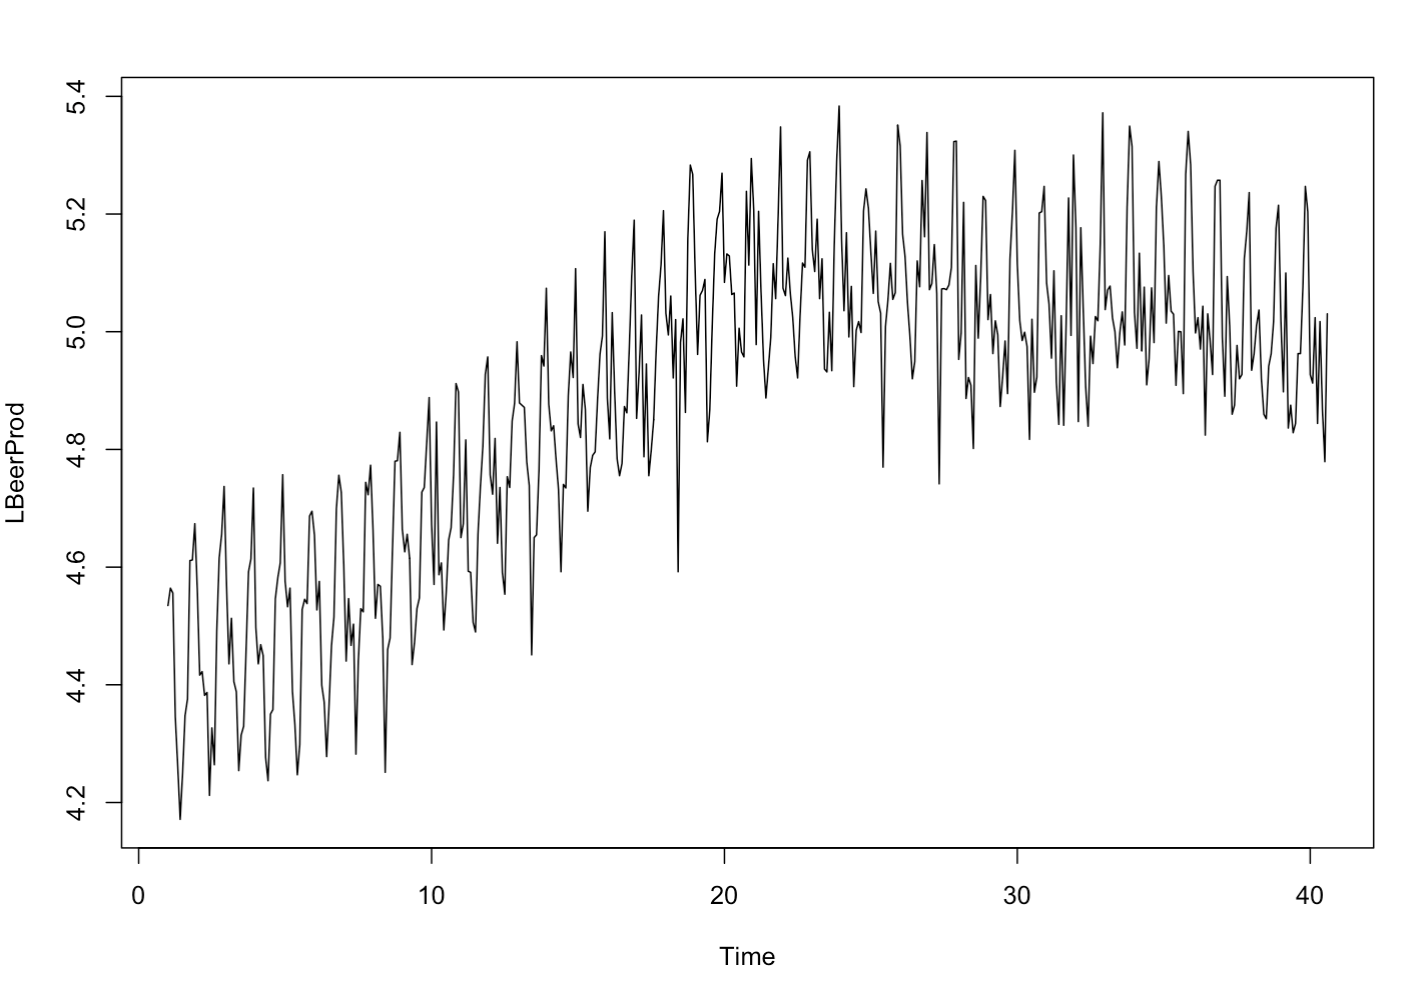
\includegraphics[scale=0.3]{Log_Series}  
    	\caption{Série avec une transformation logarithme}
    	\label{fig:sub2}
    \end{subfigure}

\caption{Comparaison série initiale et avec transformation logarithmique}
\label{fig:1}
   
\end{figure}



\vspace{5 mm}
\subsection{Élimination de la tendance et de la saisonnalité --MEILLEUR TITRE?}

\vspace{5 mm}
À partir de ces deux modèles, nous commencons par faire une différenciation $(I-B)$, soit d=1. Les sorties ACF et PACF nous affiche des pics à 12, 24, et plus, nous poussant à faire une prochaine différenciation, $(I-B^{12})$, soit D=1. Nous prenons ainsi les cas de différenciation suivants:
\begin{description}
  \item 1. d=0, D=1
  \item 2. d=1, D=1
\end{description}
\noindent 
Pour le premier cas, la série est non-stationnaire, tandis que lorsque nous prenons d=1 et D=1, nous obtenons une série stationnaire, un résultat qui est vu à la fois via les sorties ACF, PACF et à la fois grâce aux tests ADF et KPSS. Nous établirons nos prochains modèles à partir de $Y_t$ (cas non-transformé) et $YL_t$ (cas transformé)

\noindent 
Soit $(X_t)_{t\in \mathbb{Z}}$ le processus initial
\begin{align*}
Y_t &= (I-B) * (1-B^{12}) * X_t \\ 
YL_t &= (I-B) * (1-B^{12}) * log(X_t)
\end{align*}



\vspace{5 mm}
\subsection{Création de modèles}

\vspace{5 mm}
\subsubsection{Série Initial, $Y_t$)}

Nous utilisons 3 approches pour modéliser notre processus $Y_t$.

La première est une approche standard, qui permet de déterminer les p, q et P, Q qui minimiseraient le BIC. En effet, grâce à la fonction auto.arima de R nous obtenons en premier lieu SARIMA (0,1,3) X (0,1,2)[12]. Cela veut dire que notre modèle est de la forme suivante:
\begin{align*}
\theta ....ECRIRE LE MODELE
\end{align*}

Puis nous tentons de développer un autre modèle potentiel. Comme notre série semble avoir une tendance quadratique, de part sa forme concave, nous considérons une nouvelle approche qui pourrait traiter la possibilité d'endogénéité de la variable production de bière. Ainsi nous supposons que la variable pourrait être dépendante de d'autres facteurs tel que le climat. Nous créons alors le modèle SARIMAX qui est de la forme suivante:
\begin{align*}
\theta ....ECRIRE LE MODELE
\end{align*}

La dernière approche utilisée dans cet étude est la recherche du point de rupture. 
\begin{figure}[h]
	\begin{subfigure}{.5\textwidth}
  		\centering
    	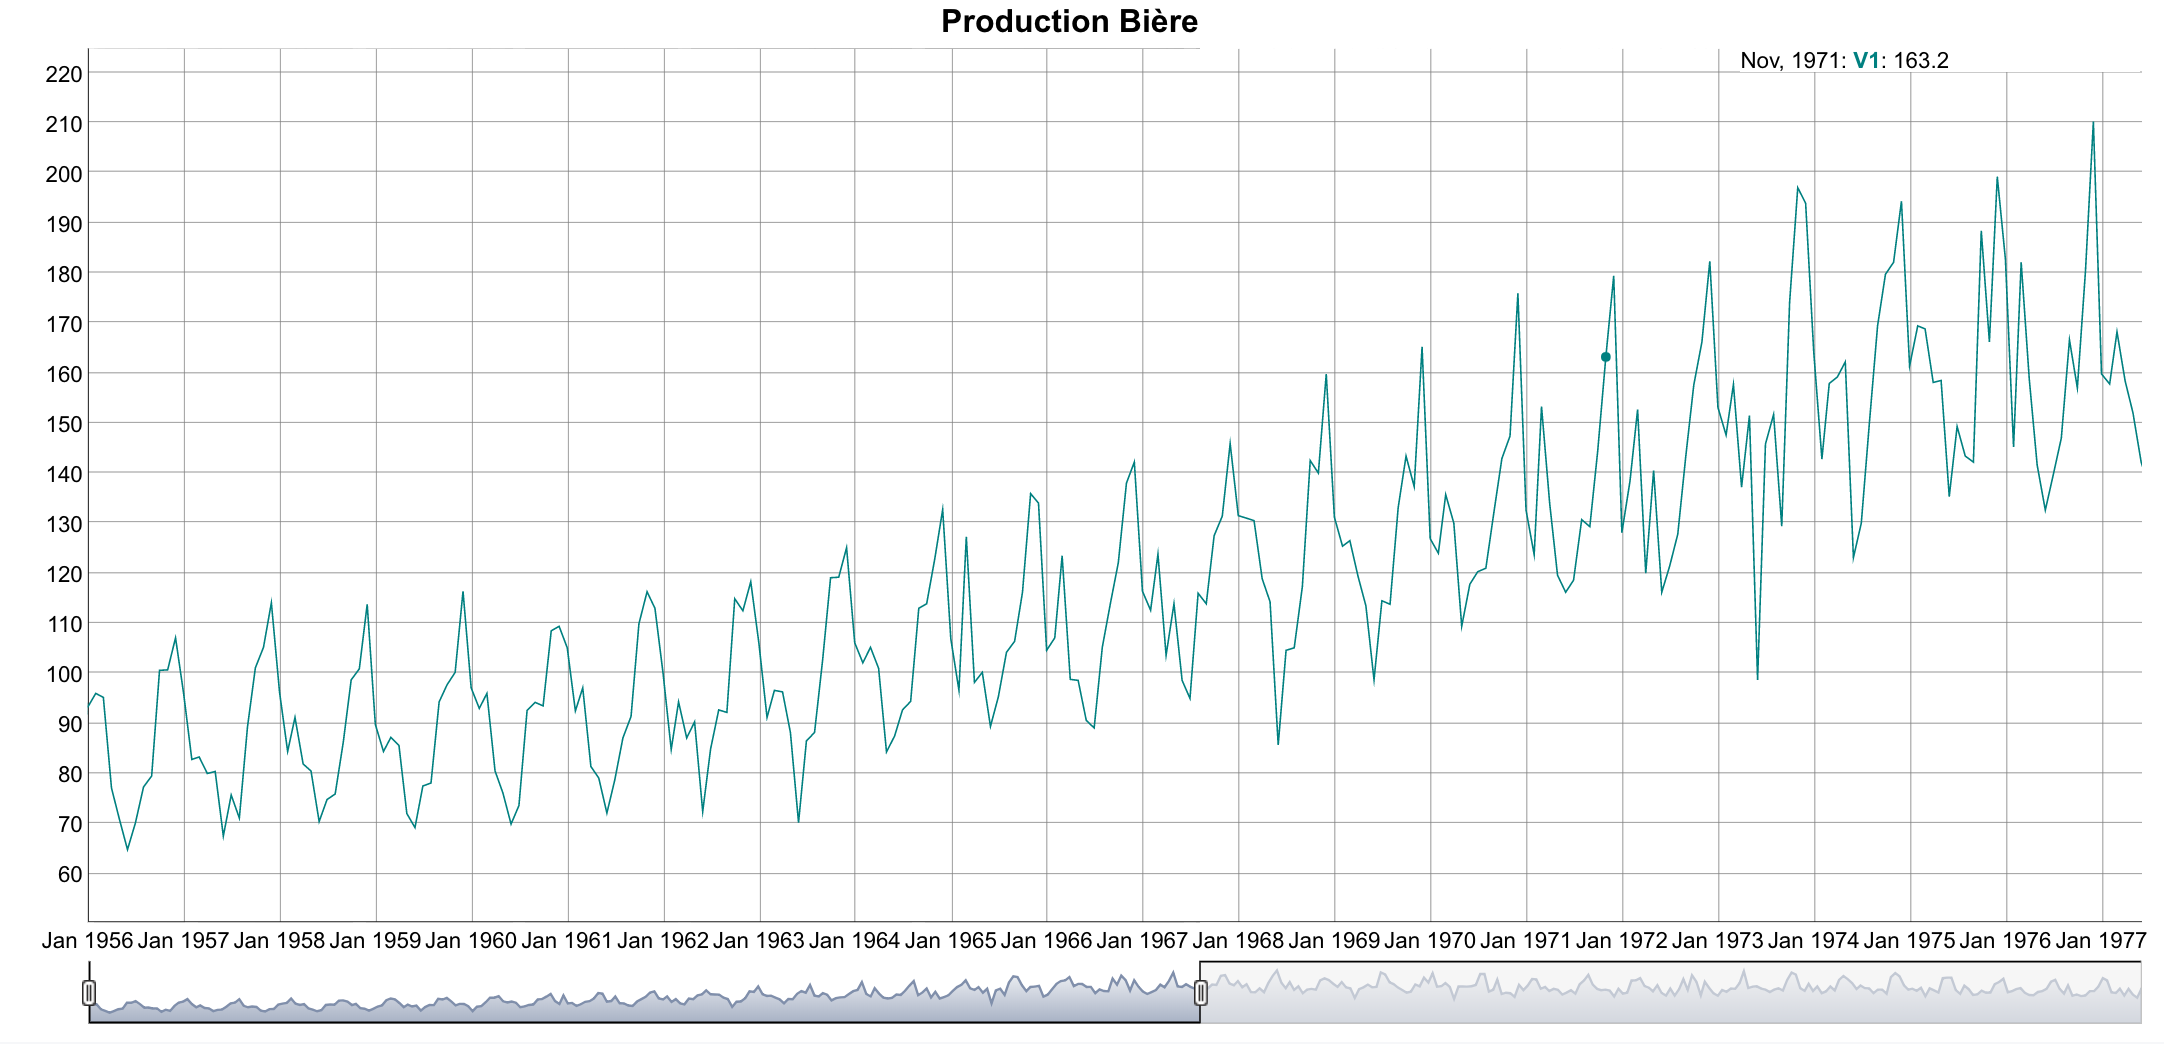
\includegraphics[scale=0.2]{rupture1}  
    	\caption{Partie à gauche de la rupture}
    	\label{fig:sub1}
    \end{subfigure}
    \begin{subfigure}{.5\textwidth}
    	\centering
    	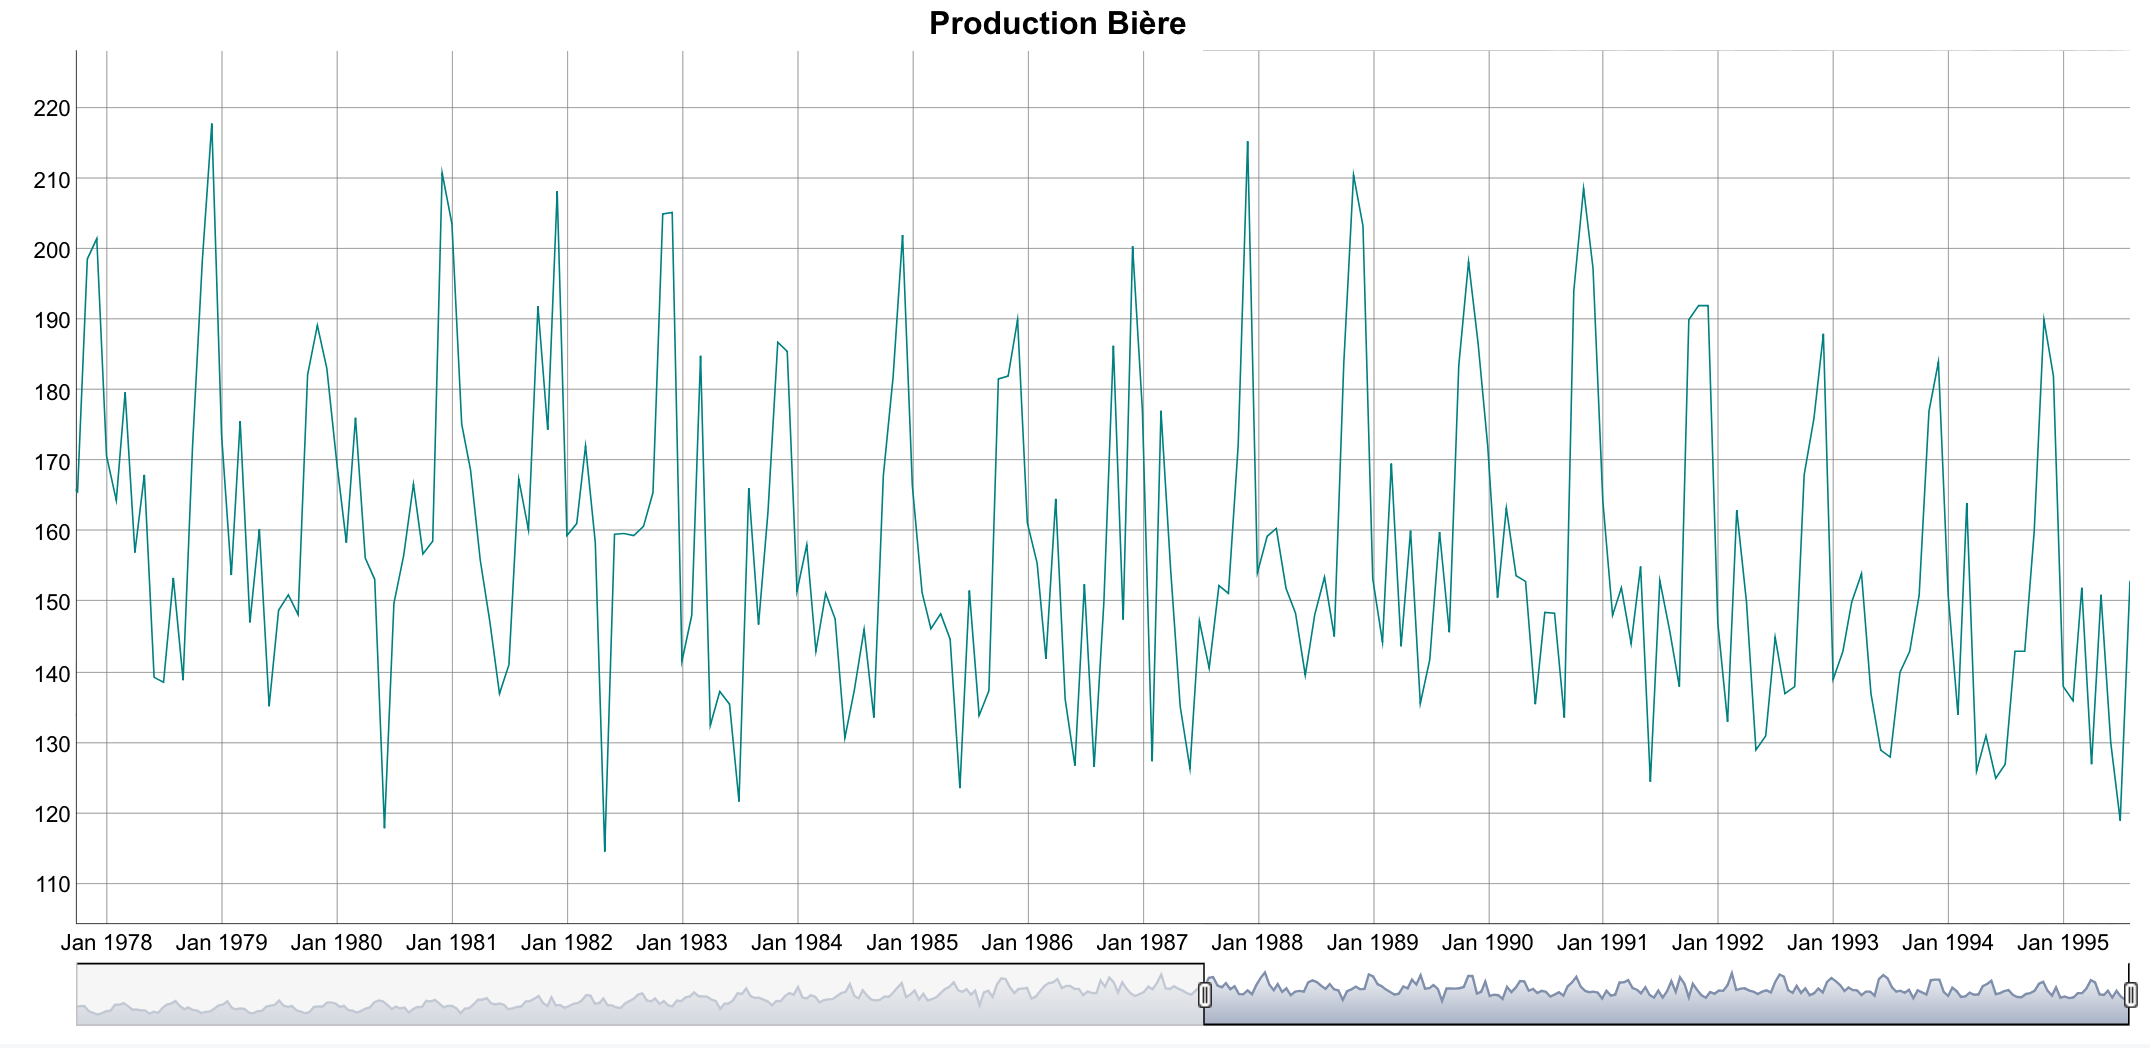
\includegraphics[scale=0.2]{rupture2}  
    	\caption{Partie à droite de la rupture}
    	\label{fig:sub2}
    \end{subfigure}

\caption{Analyse point de rupture}
\label{fig:1}
   
\end{figure}

Tout comme pour la deuxième approche nous choisissons cette méthode à cause de la tendance de la série. Nous voyons en effet, un point de rupture possible autour de 1970. Le modèle choisit par auto.arima est :
\begin{align*}
\theta ....ECRIRE LE MODELE
\end{align*}

Avant d'aller plus loin dans la comparaison des modèles, il est important de valider la qualité des résidus des modèles créés. Or, nous remarquons que bien qu'auto.arima ait sélectionné les modèles qui minimise le BIC, il ne semble pas considérer la qualité des résidus. En effet, le test de Box Jenkins nous montre que les résidus ne sont pas bruits blancs et qu'au final les modèles ne sont pas adaptés à faire les prévisions. Afin de palier à ce problème nous cherchons alors à augmenter manuellement les valeurs de p, q ainsi P et Q ce qui nous donnerait plus de flexibilité dans le modèle mais qui augmenterait le risque de paramètres non significatifs. Ainsi, pour chaque modèle créé nous effectuons un test statistique de student sur chaque coefficient. Dans chaque cas où les coefficients les plus (ELEVER-- A VALIDER QUEL TERME METTRE) sont non significatifs, une variante du modèle, ne possédant aucune variable significative est créée. Le BIC de cette dernière est comparé à celui du modèle possédant les paramètres non significatifs. Nous nous retrouvons avec les modèles suivants:

\begin{table}[h!]
  \begin{center}
    \caption{Modèles choisis}
    \label{tab:table1}
    \begin{tabular}{l|c|r} % <-- Alignments: 1st column left, 2nd middle and 3rd right, with vertical lines in between
      \ & \textbf{Modèles} & \textbf{Equations}\\
      \hline
      A & SARIMA $(4,1,4)(0,1,1)_{12}$ & $\alpha$ - à compléter\\
      B & SARIMAX $(4,0,4)(0,1,1)_{12}$& $\beta$ - à compléter\\
      C & SARIMA avec rupture $(4,1,3)(0,1,1)_{12}$ & $\gamma$ - à compléter\\
    \end{tabular}
  \end{center}
\end{table}



\vspace{5 mm}
\subsubsection{Série avec transformation logarithmique, $YL_t$)}

Nous procédons de la même façon avec le modèle logarithmique. Tout comme pour la série initiale, en faisant une différenciation, $(I-B)$ et en faisant une différenciation saisonnière $(I-B^{12})$, nous obtenons une modèle stationnaire. Le test ADF et KPSS confirme ce résultat tout comme les sorties ACF et PACF (qui nous n'affiche plus de pics cycliques). 

\begin{figure}[h]
 \centering
  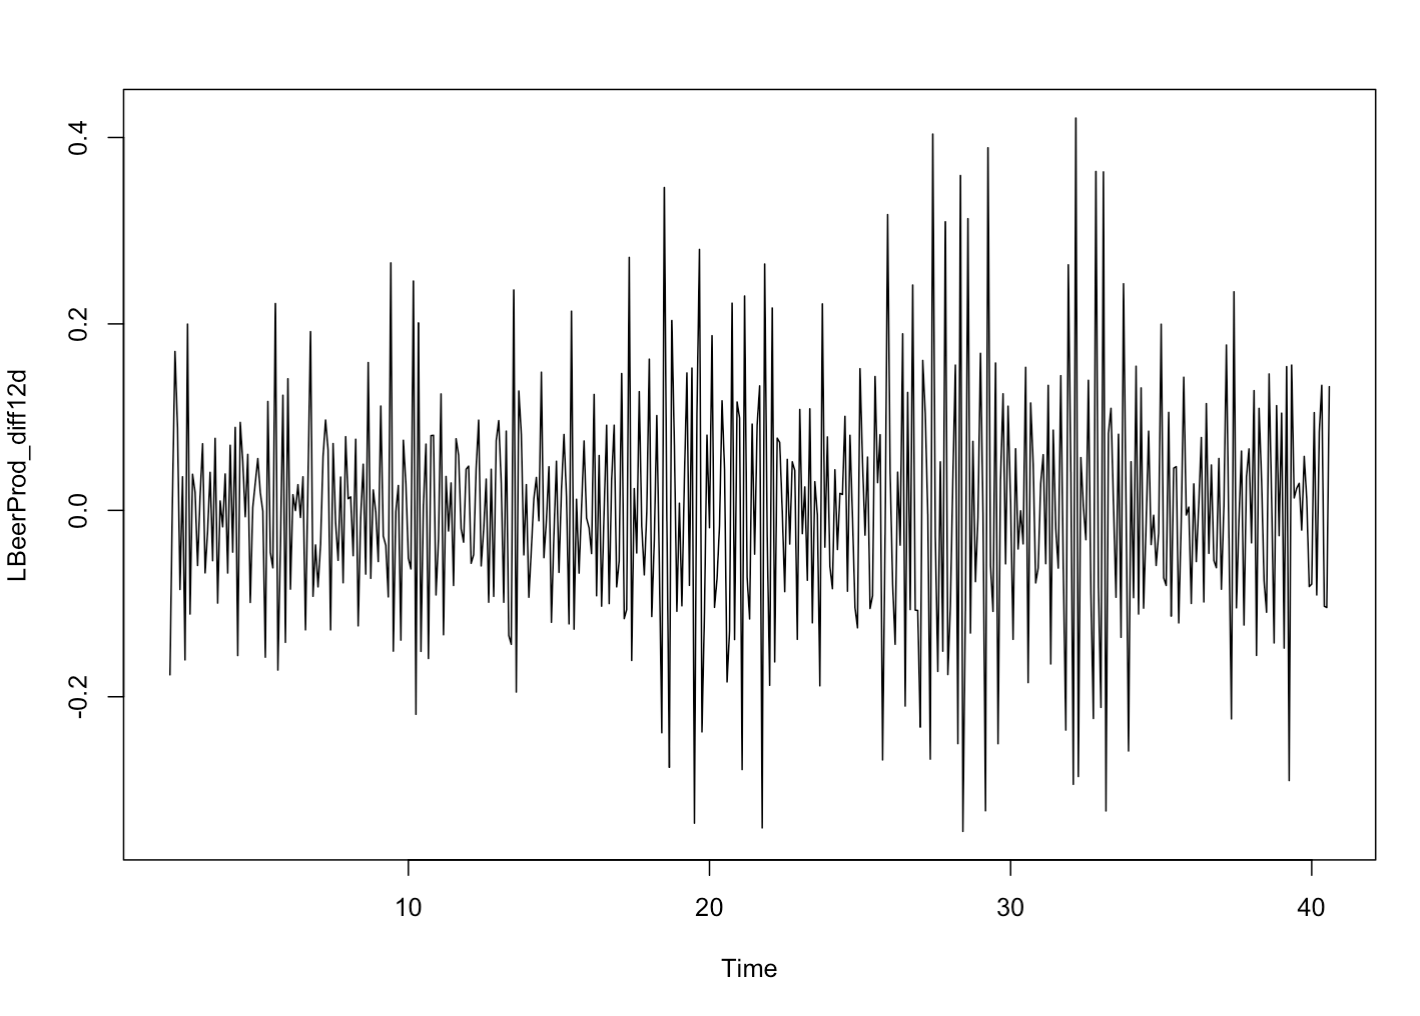
\includegraphics[scale=0.3]{Log_Avecd1D1}  
\caption{Séries logarithmique avec des différenciations, d=1, D=1 }
\label{fig:1}
\end{figure}

Dans la Figure 2, nous remarquons que la variance n'est pas tout à fait constante. En effet, elle est plus élevée autours des périodes 20 et 30. 

\vspace{5 mm}
\subsection{Analyses des résidus}
Avant de faire des prédictions avec nos modèles nous cherchons à analyser les résidus. Pour cela nous allons faire à la fois une analyse visuelle et une analyse en se basant sur les tests statistiques afin de voir si nos résidus sont bien des bruits blanc et s'ils sont gaussiens.

\subsubsection{Modèle Initial, $Y_t$}

METTRE PHOTOS CHECK UP RES du modèle avec meilleur résultat

\subsubsection{Modèle logarithme, $YL_t$}

METTRE PHOTOS CHECK UP RES du modèle avec meilleur résultat

\vspace{5 mm}
\subsection{Prédictions}

Nous cherchons maintenant à analyser la performance prédictive des modèles sur 1 an ATTENTION PREDICTION 3 ANS demandé dans le mail?. Pour le faire, une période, équivalente à 12 mois, est enlevée à partir d'août 1995. Les résultats ainsi prédits seront comparés avec les observations en utilisant le MSE, l'erreur moyenne au carré. Le modèle ayant le plus petit MSE sera le modèle sélectionné dans chacun des cas (avec et sans transformation logarithme). 


\subsubsection{Modèle Initial, $Y_t$}

Figure 4 nous affiche à la fois les prédictions des 12 derniers mois et les vrais valeurs (en noir). Nous remarquons que les 3 modèles donnent visuellement des résultats assez proche des vrais observations. Nous confirmons cela à l'aide des MSE calculés (Table 2). Nous pouvoir établir que le modèle 

\begin{figure}[h]
  		\centering
    	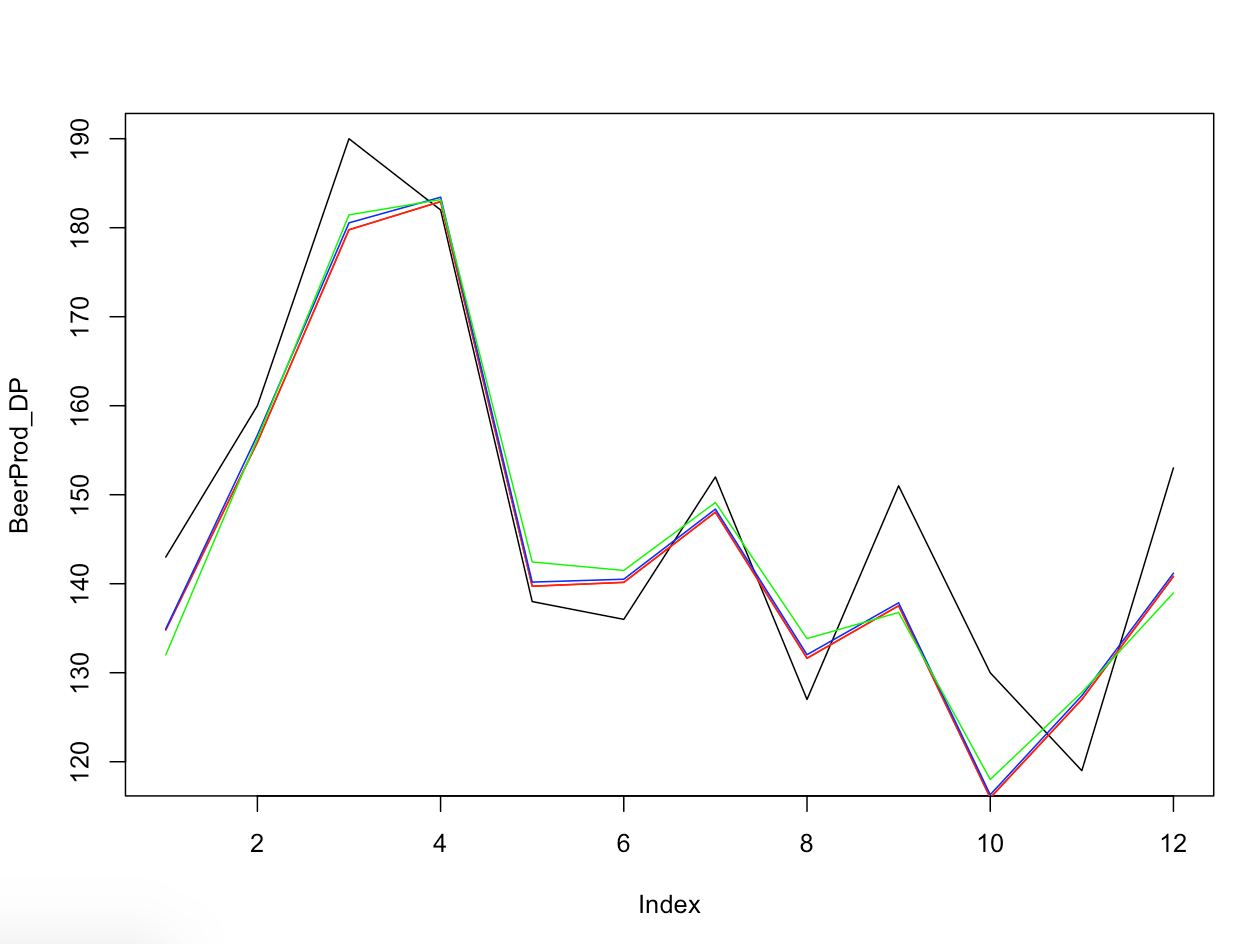
\includegraphics[scale=0.4]{Prediction_Initial}  
\caption{Prédictions des 12 derniers mois et comparaison avec les vrai valeurs à partir de la série non-transformée}
\label{fig:1}
\end{figure}

\begin{table}[h!]
  \begin{center}
    \caption{MSE}
    \label{tab:table1}
    \begin{tabular}{l|c|r} 
      \ & \textbf{Modèles} & \textbf{MSE}\\
      \hline
      A & SARIMA $(4,1,4)(0,1,1)_{12}$ & 69.82345\\
      \rowcolor{LightCyan}
      B & SARIMAX $(4,0,4)(0,1,1)_{12}$& \textbf{66.83503}\\
      C & SARIMA avec rupture $(4,1,3)(0,1,1)_{12}$ & 77.87975\\
    \end{tabular}
  \end{center}
\end{table}


\subsubsection{Modèle logarithme, $YL_t$}
Les résultats obtenus à partir des logarithmes de la séries sont affichés dans la figure 5. 
\begin{figure}[h]
  		\centering
    	\includegraphics[scale=0.4]{Prediction_Log}  
\caption{Prédictions des 12 derniers mois et comparaison avec les vrai valeurs à partir de la série transformée}
\label{fig:1}
\end{figure}

\begin{table}[h!]
  \begin{center}
    \caption{MSE}
    \label{tab:table1}
    \begin{tabular}{l|c|r} 
      \ & \textbf{Modèles} & \textbf{MSE}\\
      \hline
      D & SARIMA A AJOUTER & 0.003685328\\
      E & SARIMAX A AJOUTER & 0.003874816\\
      \rowcolor{LightCyan}
      F & SARIMA avec rupture A AJOUTER & \textbf{0.003226944}\\
    \end{tabular}
  \end{center}
\end{table}

\vspace{5 mm}
\subsection{Conclusion}

\end{document}